% !TeX program = xelatex
% =========================
% main.tex  —  Trúc giữ, người khác KHÔNG sửa file này
% Mỗi người chỉ sửa file trong thư mục chuong/ được giao.
% =========================

\documentclass[12pt,a4paper]{article}

% ============================================================
% settings.tex
% THIẾT LẬP CHUNG CHO BÁO CÁO
% ============================================================

% ------------------------------------------------------------
% KHỔ GIẤY VÀ LỀ
% ------------------------------------------------------------
\usepackage[
    a4paper,
    top=2.5cm,
    bottom=2.5cm,
    left=3cm,
    right=2cm
]{geometry}


% ------------------------------------------------------------
% FONT + TIẾNG VIỆT
% ------------------------------------------------------------
\usepackage{fontspec}
\setmainfont{TeX Gyre Termes} % Tương đương Times New Roman

\usepackage{polyglossia}
\setdefaultlanguage{vietnamese}
\setotherlanguage{english}   % cho phần tài liệu tham khảo APA


% ------------------------------------------------------------
% GIÃN DÒNG
% ------------------------------------------------------------
\usepackage{setspace}
\onehalfspacing


% ------------------------------------------------------------
% CÁC PACKAGE CẦN THIẾT
% ------------------------------------------------------------
\usepackage{graphicx}
\usepackage{tikz}
\usepackage{eso-pic}

\usepackage{xcolor}

\usepackage{booktabs}
\usepackage{tabularx}
\usepackage{array}
\usepackage{longtable}

\usepackage{enumitem}
\usepackage{titlesec}
\usepackage{tocloft}

\usepackage{caption}
\usepackage{float}

\usepackage{csquotes}
% \usepackage{microtype}   % tắt cho nhanh, tránh timeout Overleaf free

\usepackage{hyperref}
\usepackage{bookmark}


% ------------------------------------------------------------
% TÀI LIỆU THAM KHẢO APA 7
% ------------------------------------------------------------
\usepackage[
    backend=biber,
    style=apa,
    language=english,        % APA không có bản tiếng Việt
    sorting=nyt,
    natbib=true
]{biblatex}

\addbibresource{tailieu.bib}


% ------------------------------------------------------------
% MÀU
% ------------------------------------------------------------
\definecolor{UELBlue}{HTML}{1F5A94}
\definecolor{UELDarkBlue}{HTML}{174C7E}
\definecolor{GuideGray}{HTML}{6B7280}


% ------------------------------------------------------------
% HYPERLINK
% ------------------------------------------------------------
\hypersetup{
    colorlinks=true,
    linkcolor=black,
    citecolor=UELDarkBlue,
    urlcolor=UELDarkBlue,
    pdftitle={Do an cuoi ky - Phat trien Web Kinh doanh}
}


% ============================================================
% ĐỊNH DẠNG ĐOẠN VĂN
% ============================================================

\usepackage{indentfirst}          % thụt đầu dòng cả đoạn đầu tiên sau tiêu đề
\setlength{\parindent}{1.27cm}
\setlength{\parskip}{0pt}

\setlist[itemize]{
    leftmargin=1.2cm,
    itemsep=2pt,
    topsep=3pt
}

\setlist[enumerate]{
    leftmargin=1.2cm,
    itemsep=2pt,
    topsep=3pt
}


% ============================================================
% ĐÁNH SỐ MỤC
%
% I.
% II.
%   II.1.
%   II.2.
% III.
% ============================================================

\renewcommand{\thesection}{\arabic{section}}

\renewcommand{\thesubsection}{\thesection.\arabic{subsection}}

\renewcommand{\thesubsubsection}{\thesubsection.\arabic{subsubsection}}

% Cho phép đánh số đến subsubsection
\setcounter{secnumdepth}{3}


% ============================================================
% ĐỊNH DẠNG HEADING TRONG NỘI DUNG
% ============================================================

% SECTION
\titleformat{\section}
    {\bfseries\fontsize{14}{18}\selectfont}
    {\thesection.}
    {0.6em}
    {}

\titlespacing{\section}
    {0pt}
    {18pt}
    {8pt}


% SUBSECTION
\titleformat{\subsection}
    {\bfseries\fontsize{13}{17}\selectfont}
    {\thesubsection.}
    {0.6em}
    {}

\titlespacing{\subsection}
    {0pt}
    {12pt}
    {5pt}


% SUBSUBSECTION
\titleformat{\subsubsection}
    {\bfseries\fontsize{12}{16}\selectfont}
    {\thesubsubsection.}
    {0.6em}
    {}

\titlespacing{\subsubsection}
    {0pt}
    {10pt}
    {4pt}


% ============================================================
% MỤC LỤC
% STYLE GẦN GIỐNG TEMPLATE MẪU
% ============================================================

% polyglossia tự đặt lại tên theo tiếng Việt, nên phải ghi đè trong \captionsvietnamese
\gappto\captionsvietnamese{\renewcommand{\contentsname}{MỤC LỤC}}

% Chỉ hiện Section và Subsection
% Không cho 1.1.1 chen vào mục lục
\setcounter{tocdepth}{2}


% ------------------------------------------------------------
% TIÊU ĐỀ "MỤC LỤC"
% ------------------------------------------------------------

\setlength{\cftbeforetoctitleskip}{0pt}

\renewcommand{\cfttoctitlefont}{%
    \hfill\bfseries
    \fontsize{14}{18}\selectfont
}

\renewcommand{\cftaftertoctitle}{\hfill}   % căn giữa chữ MỤC LỤC
\setlength{\cftaftertoctitleskip}{0.9cm}


% ------------------------------------------------------------
% SECTION TRONG MỤC LỤC
%
% I.     MỞ ĐẦU ............................... 1
% II.    ĐỊNH HƯỚNG NGHỀ NGHIỆP ............. 2
% ------------------------------------------------------------

\renewcommand{\cftsecfont}{
    \bfseries
    \fontsize{13}{17}\selectfont
}

\renewcommand{\cftsecpagefont}{
    \bfseries
    \fontsize{13}{17}\selectfont
}

% Khoảng cách giữa các section
\setlength{\cftbeforesecskip}{0.48cm}

% Không thụt section
\setlength{\cftsecindent}{0cm}

% Khoảng dành cho I., II., III.
\setlength{\cftsecnumwidth}{1.7cm}

% Thêm dấu chấm sau số La Mã
\renewcommand{\cftsecaftersnum}{.}

% Dấu chấm nối đến số trang
\renewcommand{\cftsecleader}{
    \cftdotfill{\cftdotsep}
}


% ------------------------------------------------------------
% SUBSECTION TRONG MỤC LỤC
%
%     II.1.   Khảo sát các hướng nghề nghiệp .... 2
% ------------------------------------------------------------

\renewcommand{\cftsubsecfont}{
    \normalfont
    \fontsize{12}{16}\selectfont
}

\renewcommand{\cftsubsecpagefont}{
    \normalfont
    \fontsize{12}{16}\selectfont
}

% Khoảng cách giữa subsection
\setlength{\cftbeforesubsecskip}{0.16cm}

% Thụt vào
\setlength{\cftsubsecindent}{0.9cm}

% Khoảng dành cho II.1.
\setlength{\cftsubsecnumwidth}{1.9cm}

% Dấu "." cuối II.1.
\renewcommand{\cftsubsecaftersnum}{.}

% Dấu chấm nối
\renewcommand{\cftsubsecleader}{
    \cftdotfill{\cftdotsep}
}


% Khoảng cách giữa các dấu chấm
\renewcommand{\cftdotsep}{1.5}


% ============================================================
% BẢNG
% ============================================================

\renewcommand{\arraystretch}{1.25}

\newcolumntype{Y}{
    >{\raggedright\arraybackslash}X
}

\renewcommand{\tablename}{Bảng}
\renewcommand{\figurename}{Hình}


% ============================================================
% CAPTION
% ============================================================

\captionsetup{
    font=small,
    labelfont=bf,
    justification=centering
}


% ============================================================
% PLACEHOLDER HƯỚNG DẪN
% ============================================================

\newcommand{\placeholder}[1]{%
    {\color{GuideGray}\itshape [#1]}%
}


% ============================================================
% FOOTER
% Trang 1, Trang 2, ...
% MÀU XANH UEL
% ============================================================

\usepackage{fancyhdr}

\pagestyle{fancy}

\fancyhf{}

\fancyfoot[C]{%
    \textbf{Trang \thepage}%
}

\renewcommand{\headrulewidth}{0pt}
\renewcommand{\footrulewidth}{0pt}


% Kiểu plain cũng dùng footer giống nhau
\fancypagestyle{plain}{
    \fancyhf{}

    \fancyfoot[C]{%
        \textbf{Trang \thepage}%
    }

    \renewcommand{\headrulewidth}{0pt}
    \renewcommand{\footrulewidth}{0pt}
}
% =========================
% bia-thong-tin.tex
% CHỈ SỬA THÔNG TIN BÌA Ở FILE NÀY
% =========================

\newcommand{\CoverSemester}{Học kỳ I/2026 - 2027}
\newcommand{\CoverCourse}{PHÁT TRIỂN WEB KINH DOANH}
\newcommand{\CoverTitle}{XÂY DỰNG HỆ THỐNG WEB HỖ TRỢ PHÁT HIỆN\\VÀ XỬ LÝ ĐƠN HÀNG CÓ NGUY CƠ\\KHÔNG HÀI LÒNG ẨN}

\newcommand{\CoverSupervisor}{TS. Trần Duy Thanh}
\newcommand{\CoverCourseCode}{261BIE503002}
\newcommand{\CoverGroup}{NHÓM 1}

\newcommand{\CoverPlaceDate}{TP. HỒ CHÍ MINH, THÁNG 11/2026}



\begin{document}

% Trang 1: bìa
% =========================
% bia.tex
% Trang bìa luôn là trang đầu tiên
% =========================

\begin{titlepage}
\thispagestyle{empty}

% Nền bìa có sẵn tên trường, logo UEL và thanh xanh cuối trang
\AddToShipoutPictureBG*{%
  \AtPageLowerLeft{%
    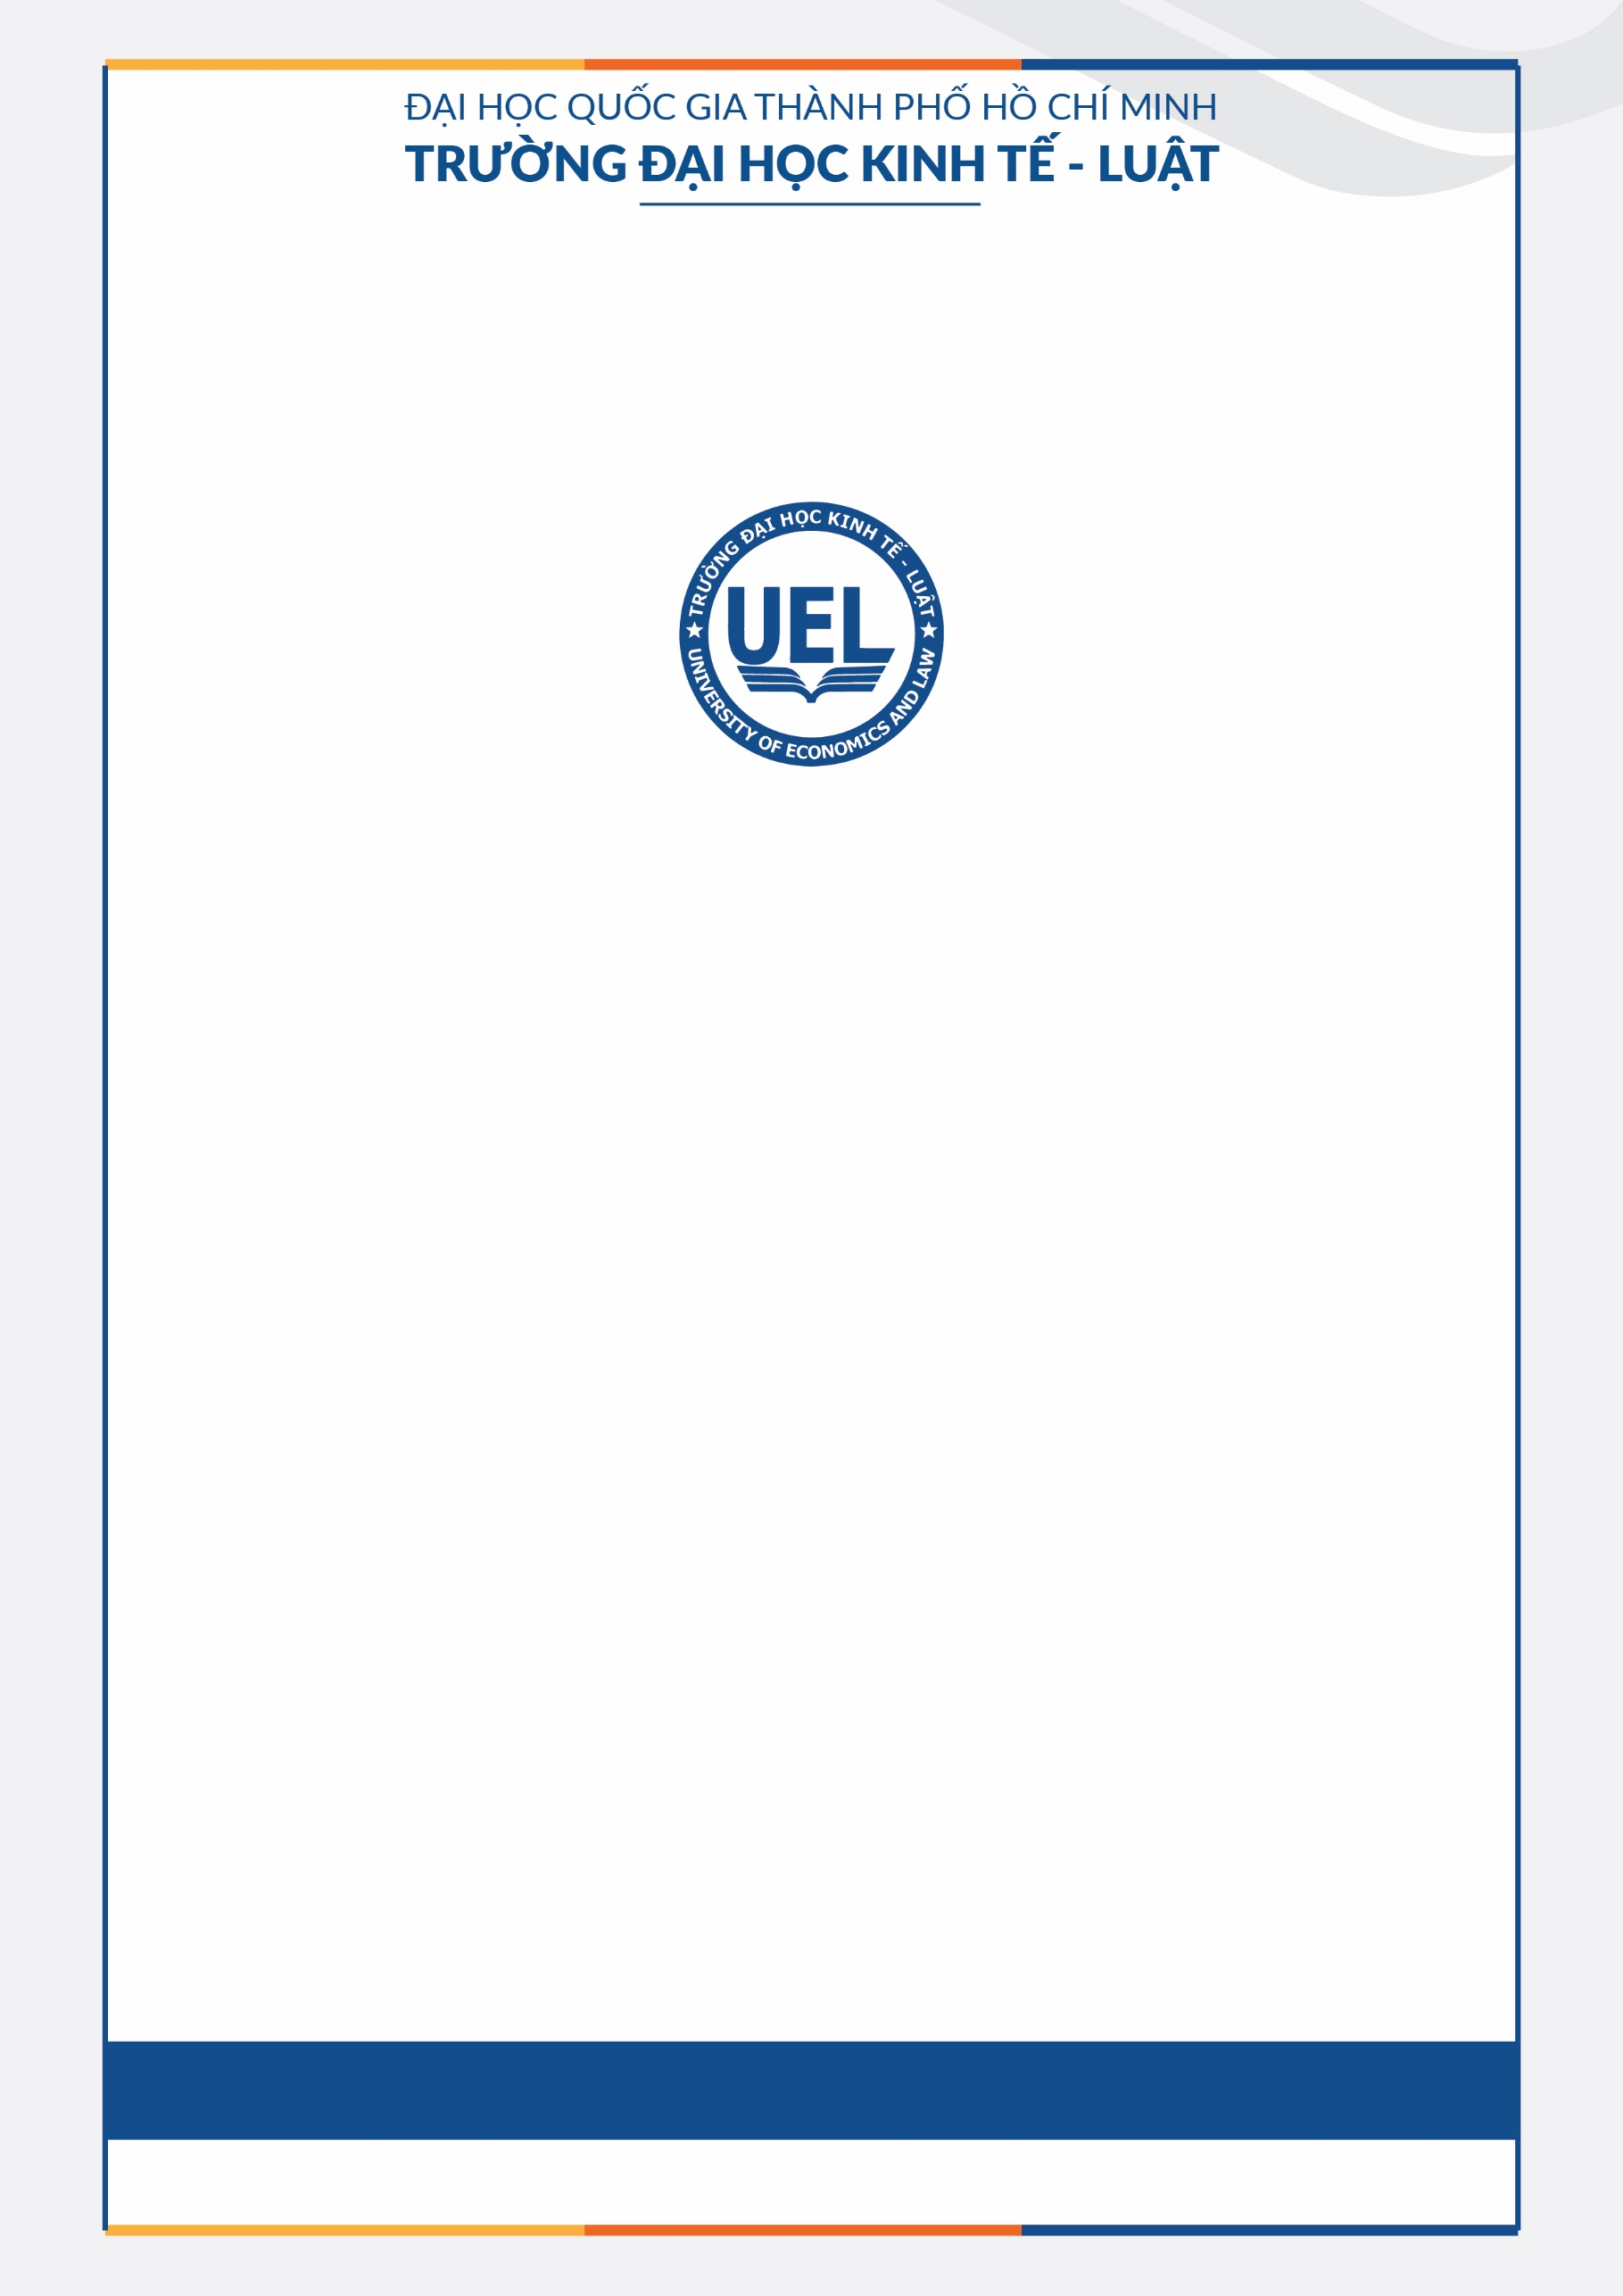
\includegraphics[width=\paperwidth,height=\paperheight]{hinh/bia-uel.jpeg}%
  }%
}

\begin{tikzpicture}[remember picture,overlay]

% Toàn bộ chữ nằm ngay dưới logo, xếp từ trên xuống
\node[
  anchor=north,
  text width=16cm,
  align=center,
  text=black,
  font=\bfseries
] at ([yshift=-10.3cm]current page.north) {%
  {\fontsize{12}{15}\selectfont \CoverSemester}\\[0.35cm]
  {\fontsize{12}{15}\selectfont MÔN HỌC: \CoverCourse}\\[0.3cm]
  {\fontsize{15}{20}\selectfont \CoverTitle}\\[0.35cm]
  {\fontsize{12}{16}\selectfont
    GVHD: \CoverSupervisor\\
    MÃ HỌC PHẦN: \CoverCourseCode\\
    NHÓM SVTH: \CoverGroup}
};

% Dòng địa điểm - thời gian ở thanh xanh cuối bìa
\node[
  anchor=center,
  text=white,
  font=\bfseries\fontsize{11.5}{14}\selectfont
] at ([yshift=2.7cm]current page.south) {\CoverPlaceDate};

\end{tikzpicture}

\null
\end{titlepage}

% Không cho hình nền bìa chạy sang trang sau
\ClearShipoutPictureBG


% Trang 2-3: danh sách thành viên + phân công
% =========================
% thanh-vien.tex
% Trang 2: danh sách thành viên + ký tên
% Trang 3: bảng phân công nhiệm vụ
% =========================

\clearpage
\thispagestyle{empty}

% Cột m{...} = căn giữa theo chiều dọc
\newcolumntype{C}[1]{>{\centering\arraybackslash}m{#1}}

\begin{center}
{\bfseries\fontsize{13}{16}\selectfont DANH SÁCH THÀNH VIÊN}
\end{center}

\vspace{0.3cm}

\begin{center}
\renewcommand{\arraystretch}{1.2}
\begin{tabular}{|C{1cm}|C{4.3cm}|C{2.6cm}|C{2.2cm}|C{3.6cm}|}
\hline
\textbf{STT} & \textbf{HỌ VÀ TÊN} & \textbf{MSSV} &
\textbf{MỨC ĐỘ ĐÓNG GÓP (\%)} & \textbf{KÝ TÊN} \\
\hline
% Ô ký tên: \rule{0pt}{1.6cm} giữ chiều cao dòng.
% Có ảnh chữ ký thì thay bằng \includegraphics[height=1.3cm]{assets/ky-ten/truc.png}
1 & [Họ tên]    & [MSSV]     & 100\% & \rule{0pt}{1.6cm} \\ \hline
2 & [Họ tên]    & [MSSV]     & 100\% & \rule{0pt}{1.6cm} \\ \hline
3 & [Họ tên]    & [MSSV]     & 100\% & \rule{0pt}{1.6cm} \\ \hline
4 & Vũ Sơn Trúc & K244161819 & 100\% & \rule{0pt}{1.6cm} \\ \hline
5 & [Họ tên]    & [MSSV]     & 100\% & \rule{0pt}{1.6cm} \\ \hline
\end{tabular}
\end{center}


% ------------------------------------------------------------
% BẢNG PHÂN CÔNG NHIỆM VỤ
% ------------------------------------------------------------

\clearpage
\thispagestyle{empty}

\begin{center}
{\bfseries\fontsize{13}{16}\selectfont BẢNG PHÂN CÔNG NHIỆM VỤ}
\end{center}

\vspace{0.3cm}

% \nhiemvu{...} = danh sách gạch đầu dòng "-" gọn trong một ô bảng
\newcommand{\nhiemvu}[1]{%
  \begin{minipage}{\linewidth}
    \vspace{4pt}
    \begin{itemize}[label=-, leftmargin=0.6cm, nosep]
      #1
    \end{itemize}
    \vspace{4pt}
  \end{minipage}%
}

\begin{center}
\renewcommand{\arraystretch}{1.2}
\begin{tabular}{|C{1cm}|C{4cm}|m{9.6cm}|}
\hline
\textbf{\textit{STT}} & \textbf{Họ và tên} & \multicolumn{1}{c|}{\textbf{Nhiệm vụ}} \\
\hline
\textbf{\textit{1}} & [Họ tên] & \nhiemvu{
  \item Nhiệm vụ 1
  \item Nhiệm vụ 2
} \\ \hline
\textbf{\textit{2}} & [Họ tên] & \nhiemvu{
  \item Nhiệm vụ 1
  \item Nhiệm vụ 2
} \\ \hline
\textbf{\textit{3}} & [Họ tên] & \nhiemvu{
  \item Nhiệm vụ 1
  \item Nhiệm vụ 2
} \\ \hline
\textbf{\textit{4}} & Vũ Sơn Trúc & \nhiemvu{
  % \item Lead nhóm, lập kế hoạch và phân công nhiệm vụ
  % \item Viết Abstract, mục 1, mục 4.1 (giao diện) và mục 6
  % \item Thiết kế và xây dựng giao diện 4 màn hình
  % \item Quay video demo
  \item Đang cập nhật
} \\ \hline
\textbf{\textit{5}} & [Họ tên] & \nhiemvu{
  \item Nhiệm vụ 1
  \item Nhiệm vụ 2
} \\ \hline
\end{tabular}
\end{center}


% Trang 4: lời cảm ơn + lời cam kết
% =========================
% loi-cam-on.tex
% Lời cảm ơn + Lời cam kết, chung một trang
% =========================

\clearpage
\thispagestyle{empty}
\setlength{\parskip}{6pt}  % cách đoạn giống mẫu, chỉ trong trang này

\begin{center}
{\bfseries\fontsize{13}{16}\selectfont LỜI CẢM ƠN}
\end{center}

Lời đầu tiên, chúng em xin gửi lời tri ân sâu sắc đến \CoverSupervisor, người đã tận tâm
hướng dẫn chúng em trong suốt học phần Phát triển Web Kinh doanh (\CoverCourseCode).

Sự chỉ dẫn tận tình của Thầy đã giúp chúng em vượt qua những khó khăn trong quá trình
thực hiện và hoàn thành đồ án này. Chúng em kính chúc Thầy luôn dồi dào sức khỏe và giữ
mãi ngọn lửa đam mê trong sự nghiệp trồng người.

Chúng em xin chân thành cảm ơn!

\vspace{0.4cm}

\begin{center}
{\bfseries\fontsize{13}{16}\selectfont LỜI CAM KẾT}
\end{center}

Nhóm chúng em xin cam đoan đồ án này là kết quả của quá trình nghiên cứu, thiết kế và
xây dựng độc lập của nhóm. Các nội dung lý thuyết được tham khảo từ các tài liệu uy tín
và đều được trích dẫn nguồn gốc rõ ràng.

Dữ liệu sử dụng trong đồ án là bộ dữ liệu công khai \textit{Brazilian E-Commerce Public
Dataset by Olist}, được khai thác đúng mục đích học tập và nghiên cứu. Các công cụ trí
tuệ nhân tạo chỉ được sử dụng ở vai trò hỗ trợ, trong phạm vi cho phép của giảng viên.
Chúng em cam kết không sao chép hay sử dụng trái phép bất kỳ dữ liệu nào.

Nhóm xin chịu hoàn toàn trách nhiệm trước Thầy và Nhà trường về tính trung thực của bài
làm này.

\vspace{0.4cm}

\begin{flushright}
\bfseries\itshape
TP. Hồ Chí Minh, ngày 06 tháng 11 năm 2026\\[0.2cm]
Nhóm 1.
\end{flushright}

\setlength{\parskip}{0pt}


% Mục lục, không hiện số trang
\clearpage
\pagestyle{empty}
\pagenumbering{gobble}
\tableofcontents
\thispagestyle{empty}   % trang mục lục không in số trang
\clearpage

% Nội dung chính, bắt đầu từ trang 1
\pagestyle{fancy}
\pagenumbering{arabic}
\setcounter{page}{1}

% =========================
% chuong/00-tom-tat.tex
% TÓM TẮT (Abstract)
% =========================

\section*{TÓM TẮT}
\addcontentsline{toc}{section}{TÓM TẮT}

Trong thương mại điện tử, tỉ lệ giao hàng đúng hạn thường được xem là thước đo chính của chất lượng
dịch vụ. Tuy nhiên, phân tích bộ dữ liệu công khai của Olist cho thấy 66,3\% đơn bị chấm 1 hoặc 2 sao
lại là đơn đã giao đúng hạn. Nhóm gọi hiện tượng này là sự không hài lòng ẩn và xây dựng một hệ thống
web giúp nhân viên chăm sóc khách hàng phát hiện và xử lý sớm những đơn có nguy cơ, trước khi khách
để lại đánh giá. Hệ thống nhận kết quả dự đoán rủi ro từ mô hình học máy, biến mỗi đơn có nguy cơ
thành một case trong hàng đợi ưu tiên, hỗ trợ nhận và giao việc theo giới hạn khối lượng, ghi nhận
từng lần liên lạc kèm minh chứng, đóng case với kết quả bắt buộc, và cho quản lý theo dõi tổng quan,
ra quyết định, cấu hình tham số, truy vết mọi thao tác. Nhóm phân tích nghiệp vụ bằng BPMN, FDD, DFD,
Use Case, thiết kế cơ sở dữ liệu PostgreSQL, xây dựng máy chủ API bằng FastAPI và giao diện chín màn
hình bằng HTML, CSS, JavaScript thuần, đóng gói bằng Docker Compose. Hệ thống được kiểm thử hai
đợt với dữ liệu 100 đơn Olist thật; các lỗi của đợt đầu đã được sửa và kiểm lại. Kết quả cho thấy có thể chuyển
một điểm số dự đoán thành quy trình chăm sóc khách hàng có trách nhiệm rõ ràng và truy vết được.

\noindent\textbf{Từ khóa:} thương mại điện tử, sự không hài lòng ẩn, chăm sóc khách hàng chủ động,
hệ thống hỗ trợ ra quyết định, ứng dụng web.

% =========================
% chuong/01-gioi-thieu.tex  —  người viết: Trúc
% MỤC 1. GIỚI THIỆU
% Số liệu mô tả phải được tái lập từ pipeline version hóa trước khi nộp báo cáo.
% Cohort: delivered, order_delivered_customer_date <= order_estimated_delivery_date.
% Nhãn: review_score 1--2; chính sách multiple-review hiện giữ câu trả lời mới nhất
% và phải được chốt trong luận văn. Không dùng số liệu từ lần đếm theo chính sách khác.
% =========================

\section{GIỚI THIỆU}

% ------------------------------------------------------------
\subsection{Bối cảnh và lý do thực hiện dự án}

Trong thương mại điện tử, điểm đánh giá của khách hàng là một trong những thông tin
người mua xem trước khi ra quyết định. Nghiên cứu trên hơn 15 triệu đơn hàng của nền
tảng Tmall cho thấy trải nghiệm giao hàng ảnh hưởng đến điểm đánh giá, và điểm đánh giá
đó có liên hệ với khả năng mua hàng của những khách đến sau và doanh số người bán
\parencite{deshpande2023}. Vì vậy, review thấp là một tín hiệu dịch vụ đáng theo dõi,
nhưng dữ liệu quan sát không đủ để quy trực tiếp thành doanh thu bị mất.

Giao hàng trễ là nguyên nhân thường được nhắc đến nhất. \textcite{ravula2023} cho thấy
khách hàng chấm điểm thấp hơn rõ rệt khi đơn đến trễ, trong khi giao sớm chỉ được cộng
thêm rất ít. Do đó, các doanh nghiệp thường theo dõi tỉ lệ giao đúng hạn như một chỉ số
chính của chất lượng dịch vụ. Tuy vậy, giao nhanh hơn chưa chắc làm khách hài lòng hơn:
khi nhà bán lẻ tách đơn để giao nhanh từng phần, sự phiền toái khi nhận nhiều lần giao
có thể triệt tiêu lợi ích của tốc độ và làm giảm việc mua lại \parencite{brylla2022}.

Tuy nhiên, khi phân tích bộ dữ liệu công khai của Olist \parencite{olist2018}, nhóm nhận
thấy vẫn tồn tại các đơn được giao trước hoặc đúng ngày dự kiến nhưng nhận review 1 hoặc
2 sao. Tỷ lệ và số lượng chính thức phải được tái lập từ pipeline theo đúng chính sách
multiple-review đã version hóa trước khi đưa vào báo cáo kết quả. Quan sát này cho thấy
``đúng hạn'' không đồng nghĩa với ``hài lòng'' và tạo ra một nhóm case mà quy tắc chỉ theo
dõi giao trễ sẽ bỏ sót.

Nhóm gọi hiện tượng này là \textit{sự không hài lòng ẩn} (hidden dissatisfaction): khách
hàng không hài lòng dù đơn hàng không có dấu hiệu bất thường nào trên các chỉ số vận hành.
Đây là lý do nhóm chọn đề tài xây dựng một hệ thống web giúp doanh nghiệp nhận diện và xử
lý sớm những đơn hàng này.

% ------------------------------------------------------------
\subsection{Vấn đề cần giải quyết}

Các nghiên cứu dự đoán sự hài lòng trên dữ liệu Olist chủ yếu tập trung so sánh độ chính
xác của các mô hình và dừng lại ở việc gán nhãn cho từng đơn hàng \parencite{orman2026}.
Kết quả dạng này khó được sử dụng trực tiếp trong vận hành, vì nhân viên chăm sóc khách
hàng cần biết đơn nào cần liên hệ trước, vì sao đơn đó có nguy cơ, và nên làm gì tiếp theo.
Ngay cả khi có điểm dự đoán, việc chọn đơn nào để xử lý trước khi năng lực có hạn cũng
không đơn giản: một nghiên cứu gần đây trên ba bộ dữ liệu, trong đó có Olist, cho thấy
xếp hạng bằng mô hình học máy không phải lúc nào cũng tốt hơn quy tắc đơn giản là ưu tiên
đơn có giá trị cao nhất \parencite{li2026}. Vì vậy, người dùng cần một công cụ hiển thị
đồng thời mức rủi ro và các thông tin nghiệp vụ để tự đưa ra quyết định.

Thời điểm can thiệp cũng quan trọng. Trong ngành hàng không, việc chủ động thông báo cho
hành khách trước khi sự cố xảy ra giúp giảm đáng kể phản hồi tiêu cực trên mạng so với
xử lý khi sự cố đã diễn ra \parencite{nazifi2021}. Tương tự, nếu doanh nghiệp liên hệ
khách hàng trước khi họ để lại đánh giá, vấn đề có cơ hội được giải quyết sớm hơn.

Từ góc độ hệ thống thông tin, nhóm xác định ba vấn đề cụ thể:

\begin{itemize}
    \item Chưa có công cụ tập hợp các đơn giao đúng hạn nhưng có nguy cơ bị đánh giá thấp
    thành một danh sách ưu tiên để nhân viên xử lý trước khi khách hàng đánh giá.
    \item Kết quả dự đoán, nếu chỉ ở dạng điểm số trong một tệp dữ liệu, không kèm lý do và
    hành động đề xuất, nên người không chuyên về dữ liệu khó sử dụng.
    \item Không có nơi ghi nhận ai đã xử lý đơn nào và kết quả ra sao, nên doanh nghiệp không
    theo dõi và đánh giá được hiệu quả của việc chăm sóc khách hàng.
\end{itemize}

Từ đó, câu hỏi đặt ra cho dự án là: \textit{cần xây dựng hệ thống web như thế nào để kết quả
dự đoán rủi ro được chuyển thành danh sách ưu tiên, lời giải thích và hành động cụ thể mà
nhân viên chăm sóc khách hàng có thể sử dụng hằng ngày?}

% ------------------------------------------------------------
\subsection{Mục tiêu của dự án}

\textbf{Mục tiêu tổng quát:} xây dựng một hệ thống web hỗ trợ nhân viên chăm sóc khách hàng
phát hiện và xử lý các đơn hàng giao đúng hạn nhưng có nguy cơ nhận đánh giá tiêu cực.

\textbf{Mục tiêu cụ thể:}

\begin{enumerate}
    \item Phân tích và thiết kế hệ thống thông qua các sơ đồ Use Case, DFD, BPMN và ERD.
    \item Thiết kế cơ sở dữ liệu dựa trên 9 bảng dữ liệu Olist, bổ sung các bảng do hệ thống
    tạo ra để lưu kết quả dự đoán, hành động xử lý và người dùng.
    \item Xây dựng bốn màn hình chính: danh sách đơn cần ưu tiên (Risk Queue), chi tiết lý do
    rủi ro của từng đơn (Order Detail), ghi nhận và theo dõi xử lý (Action Tracking), và
    minh bạch nguồn dữ liệu (Data Quality).
    \item Tích hợp output ML cấp product item và kết quả tổng hợp cấp order theo \texttt{max-v1},
    kèm model version, threshold version, aggregation rule và các yếu tố liên quan.
    \item Đảm bảo giao diện hiển thị được trên máy tính, máy tính bảng và điện thoại.
\end{enumerate}

% ------------------------------------------------------------
\subsection{Phạm vi và giới hạn của dự án}

\textbf{Phạm vi:}

\begin{itemize}
    \item Dữ liệu: bộ dữ liệu công khai Brazilian E-Commerce Public Dataset by Olist, gồm
    99.441 đơn hàng từ tháng 9/2016 đến tháng 10/2018, chia thành 9 bảng có quan hệ với nhau.
    \item Đối tượng phân tích: các đơn đã giao đến khách và được giao trước hoặc đúng ngày dự
    kiến. Đơn giao trễ không thuộc phạm vi vì nguyên nhân không hài lòng đã rõ.
    \item Người dùng: nhân viên chăm sóc khách hàng và người quản lý của doanh nghiệp.
    \item Sản phẩm: hệ thống web ở mức nguyên mẫu (prototype), chạy được với dữ liệu thật
    của Olist và kết quả dự đoán rủi ro.
\end{itemize}

\textbf{Giới hạn:}

\begin{itemize}
    \item Báo cáo web không tự huấn luyện lại mô hình; nó nhận artifact từ pipeline ML của
    dự án và tập trung vào contract, trình bày, sử dụng và lưu trữ kết quả.
    \item Olist chỉ có review cấp order, không có nhãn riêng cho product item. Mỗi item kế
    thừa nhãn order; score item chỉ phản ánh rủi ro của order trong bối cảnh item và không
    chứng minh item gây ra review thấp.
    \item Chỉ một phần khách hàng chủ động viết đánh giá, nên những người đánh giá không đại
    diện đầy đủ cho toàn bộ người mua \parencite{li2008}. Đơn không có đánh giá không được
    xem là đơn khách hài lòng.
    \item Khách hàng có rủi ro cao nhất chưa chắc là nhóm phản hồi tốt nhất với việc chăm sóc
    \parencite{ascarza2018}. Vì vậy, hành động đề xuất trên hệ thống chỉ mang tính tham khảo,
    quyết định cuối cùng do nhân viên đưa ra, và dự án không đánh giá hiệu quả thực tế của
    việc liên hệ khách hàng.
    \item Dữ liệu thuộc thị trường Brazil giai đoạn 2016--2018. Kết quả không được xem là áp
    dụng trực tiếp cho thị trường Việt Nam hay thời điểm hiện tại.
    \item Hệ thống chỉ ghi nhận hành động xử lý, không tích hợp gọi điện hay gửi email thật
    đến khách hàng.
\end{itemize}

% ------------------------------------------------------------
\subsection{Phương pháp nghiên cứu và cách tiếp cận}

Nhóm tiếp cận dự án theo hướng phát triển hệ thống thông tin hỗ trợ ra quyết định, gồm
các bước sau:

\begin{enumerate}
    \item \textbf{Khảo sát dữ liệu:} tìm hiểu cấu trúc 9 bảng Olist và đo các số liệu nền
    như tỉ lệ đơn giao đúng hạn bị đánh giá thấp để xác định vấn đề.
    \item \textbf{Phân tích yêu cầu:} xác định người dùng, nhu cầu thông tin và các chức năng
    cần có, thể hiện qua sơ đồ Use Case, DFD và BPMN.
    \item \textbf{Thiết kế:} thiết kế cơ sở dữ liệu (ERD), thống nhất cấu trúc dữ liệu kết
    quả dự đoán, và thiết kế giao diện bằng wireframe trên Figma trước khi lập trình.
    \item \textbf{Xây dựng và tích hợp:} xây dựng giao diện bằng HTML, CSS và JavaScript, đọc
    dữ liệu ở định dạng JSON, kết nối với cơ sở dữ liệu và nạp kết quả dự đoán rủi ro.
    \item \textbf{Kiểm thử và đánh giá:} kiểm tra các chức năng chính và hiển thị trên ba kích
    thước màn hình, sau đó đối chiếu kết quả với các mục tiêu đã đặt ra.
\end{enumerate}

Chi tiết về dữ liệu, công nghệ sử dụng và cách đánh giá được trình bày ở mục 3.

% =========================
% chuong/02-co-so-ly-thuyet.tex
% MỤC 2. CƠ SỞ LÝ THUYẾT
% Tài liệu: ưu tiên từ 2021, KHÔNG dùng MDPI, Frontiers, Hindawi. DOI đã kiểm qua Crossref ngày 05/11/2026.
% =========================

\section{CƠ SỞ LÝ THUYẾT}

% ------------------------------------------------------------
\subsection{Tổng quan các khái niệm liên quan}

\subsubsection{Ứng dụng web trong hoạt động kinh doanh thương mại điện tử}

Trong thương mại điện tử, ứng dụng web có hai nhóm vai trò. Nhóm thứ nhất hướng tới khách hàng:
website bán hàng, trang sản phẩm, giỏ hàng, thanh toán. Nhóm thứ hai phục vụ vận hành nội bộ: các
ứng dụng web quản lý đơn hàng, chăm sóc khách hàng, báo cáo cho quản lý. Nhóm thứ hai không trực tiếp
tạo ra đơn hàng nhưng quyết định chất lượng dịch vụ sau bán, từ đó ảnh hưởng tới đánh giá, uy tín và
khả năng khách quay lại mua.

So với phần mềm cài trên máy, nền tảng web phù hợp cho nghiệp vụ vận hành ở bốn điểm: người dùng chỉ
cần trình duyệt, nhiều người làm việc cùng lúc trên cùng một dữ liệu, quyền truy cập được phân theo
vai trò, và doanh nghiệp cập nhật hệ thống một lần cho mọi người dùng. Hệ thống trong đồ án thuộc nhóm
thứ hai: một ứng dụng web nội bộ giúp bộ phận chăm sóc khách hàng biết nên liên hệ ai trước, ghi lại
đã làm gì, và giúp quản lý theo dõi chất lượng chăm sóc qua các con số.

\subsubsection{Sự hài lòng của khách hàng và đánh giá trực tuyến}

Sự hài lòng của khách hàng là mức độ trải nghiệm thực tế đáp ứng hoặc vượt kỳ vọng của khách
hàng đối với sản phẩm và dịch vụ. Trong thương mại điện tử, sự hài lòng được thể hiện rõ nhất qua
điểm đánh giá sau khi nhận hàng. Điểm đánh giá vừa là phản hồi cho doanh nghiệp, vừa là thông tin
công khai mà người mua sau tham khảo, nên một đánh giá thấp ảnh hưởng trực tiếp đến doanh số của
người bán \parencite{deshpande2023}. Tuy nhiên, chỉ một phần khách hàng chủ động viết đánh giá, và
những người viết thường có trải nghiệm rất tốt hoặc rất tệ \parencite{li2008}. Vì vậy, đánh giá là
tín hiệu có giá trị nhưng không đại diện đầy đủ cho toàn bộ khách hàng.

\subsubsection{Sự không hài lòng ẩn}

Trong đồ án này, \textit{sự không hài lòng ẩn} (hidden dissatisfaction) được hiểu là trường hợp
khách hàng chấm 1 hoặc 2 sao cho một đơn hàng mà các chỉ số vận hành không báo bất thường, cụ thể là
đơn đã được giao trước hoặc đúng ngày dự kiến. Những đơn này không xuất hiện trong các báo cáo theo
dõi giao trễ, nên doanh nghiệp chỉ biết khách không hài lòng khi đánh giá đã được đăng. Như đã trình
bày ở mục 1.1, nhóm này chiếm 66,3\% số đơn bị chấm thấp trong dữ liệu Olist.

\subsubsection{Khôi phục dịch vụ và chăm sóc khách hàng chủ động}

Khôi phục dịch vụ (service recovery) là các hành động doanh nghiệp thực hiện để khắc phục một trải
nghiệm không tốt của khách hàng. \textcite{vanvaerenbergh2019} mô tả khôi phục dịch vụ như một hành
trình gồm ba giai đoạn: trước khi khách phàn nàn, trong lúc xử lý và sau khi xử lý; doanh nghiệp có
thể can thiệp ngay từ giai đoạn đầu thay vì chờ khách lên tiếng. Nghiên cứu của
\textcite{nazifi2021} trong ngành hàng không cho thấy chủ động liên hệ khách trước khi sự cố được
khách cảm nhận giúp giảm phản hồi tiêu cực trên mạng rõ rệt so với xử lý bị động. Hệ thống trong đồ
án áp dụng tinh thần này: nhân viên liên hệ khách có nguy cơ không hài lòng trước khi họ để lại đánh
giá.

\subsubsection{Hệ thống hỗ trợ ra quyết định và vai trò của con người}

Hệ thống hỗ trợ ra quyết định (Decision Support System) là hệ thống thông tin giúp người dùng ra
quyết định dựa trên dữ liệu và mô hình, nhưng quyết định cuối cùng vẫn thuộc về con người. Đây là
điểm quan trọng khi hệ thống dùng kết quả của mô hình học máy. Tổng quan của \textcite{burton2020}
cho thấy người dùng thường e ngại thuật toán (algorithm aversion), nhất là
sau khi thấy thuật toán sai. \textcite{dietvorst2018} chỉ ra người dùng chấp nhận thuật toán chưa
hoàn hảo hơn nếu họ được điều chỉnh kết quả, dù chỉ một chút. Thí nghiệm của \textcite{bansal2021}
cho thấy việc kèm lời giải thích không tự động làm đội người và AI ra quyết định tốt hơn, vì người dùng
có thể tin theo cả những gợi ý sai. Từ các kết quả này, nhóm thiết kế hệ thống để điểm rủi ro chỉ là
căn cứ ưu tiên: nhân viên đọc yếu tố liên quan, tự liên hệ khách, tự ghi kết quả, và giao diện luôn
nhắc rằng điểm số không phải kết luận.

\subsubsection{Bảng điều khiển (dashboard)}

\textcite{sarikaya2019} phân loại dashboard theo mục đích sử dụng và chỉ ra dashboard vận hành cần
giúp người xem nhận ra việc phải làm, chứ không chỉ hiển thị số liệu. \textcite{bach2023} tổng hợp
các mẫu thiết kế dashboard, trong đó có nguyên tắc đặt chỉ số quan trọng nhất ở vị trí dễ thấy, nhóm
các chỉ số liên quan và cho phép đi từ con số tổng hợp tới dữ liệu chi tiết. Trang Tổng quan của hệ
thống áp dụng các nguyên tắc này: số đơn mức cao chờ giao được đặt đầu tiên, mỗi con số đều bấm được
để mở danh sách đơn đã lọc sẵn.

% ------------------------------------------------------------
\subsection{Các nghiên cứu và dự án liên quan}

Nhóm chia các nghiên cứu liên quan thành bốn hướng.

\textbf{Giao hàng và đánh giá của khách hàng.} \textcite{deshpande2023} dùng dữ liệu hơn 15 triệu
đơn trên Tmall và chứng minh hiệu quả giao hàng ảnh hưởng tới điểm đánh giá, từ đó ảnh hưởng tới
doanh số. \textcite{ravula2023} cho thấy giao trễ làm điểm giảm mạnh, còn giao sớm chỉ được cộng rất
ít. \textcite{brylla2022} chỉ ra giao nhanh bằng cách tách đơn có thể phản tác dụng. Các nghiên cứu
này giải thích vì sao giao đúng hạn là cần nhưng chưa đủ, nhưng không đưa ra công cụ để doanh nghiệp
xử lý từng đơn.

\textbf{Dự đoán sự hài lòng trên dữ liệu Olist.} \textcite{orman2026} so sánh các mô hình học sâu để
phân loại đơn hài lòng và không hài lòng. Hướng này tập trung vào độ chính xác của mô hình và dừng ở
nhãn dự đoán; kết quả chưa được đưa vào một quy trình mà nhân viên có thể dùng hằng ngày.

\textbf{Ưu tiên xử lý khi nguồn lực có hạn.} \textcite{ascarza2018} chứng minh khách hàng có rủi ro
cao nhất chưa chắc là nhóm phản hồi tốt nhất với việc chăm sóc. \textcite{lemmens2020} đề xuất chọn
khách để can thiệp theo lợi nhuận kỳ vọng thay vì chỉ theo xác suất rời bỏ. \textcite{li2026} cho thấy
xếp hạng bằng học máy không phải lúc nào cũng tốt hơn quy tắc đơn giản. Bài học cho hệ thống là danh
sách ưu tiên phải hiển thị thêm thông tin nghiệp vụ (SLA, thời gian chờ, người bán) để con người tự
điều chỉnh, và phải ghi lại kết quả xử lý để sau này đánh giá được hiệu quả.

\textbf{Can thiệp chủ động và cộng tác người--máy.} \textcite{nazifi2021} và
\textcite{vanvaerenbergh2019} ủng hộ can thiệp sớm; \textcite{dietvorst2018} và
\textcite{bansal2021} cho thấy người dùng cần quyền điều chỉnh và cần hiểu giới hạn của gợi ý.

Bảng~\ref{tab:nghien-cuu} tóm tắt các nghiên cứu chính và phần hệ thống kế thừa.

{\small
\renewcommand{\arraystretch}{1.25}
\begin{longtable}{|>{\raggedright\arraybackslash}p{2.4cm}|>{\raggedright\arraybackslash}p{4.1cm}|>{\raggedright\arraybackslash}p{3.4cm}|>{\raggedright\arraybackslash}p{4.3cm}|}
\caption{Các nghiên cứu liên quan và phần hệ thống kế thừa}\label{tab:nghien-cuu}\\
\hline
\textbf{Nghiên cứu} & \textbf{Kết quả chính} & \textbf{Hạn chế với bài toán} & \textbf{Hệ thống kế thừa} \\ \hline
\endfirsthead
\hline
\textbf{Nghiên cứu} & \textbf{Kết quả chính} & \textbf{Hạn chế với bài toán} & \textbf{Hệ thống kế thừa} \\ \hline
\endhead
\textcite{deshpande2023} & Giao hàng ảnh hưởng tới điểm đánh giá và doanh số & Không xét đơn giao đúng hạn mà vẫn bị chê & Lý do cần xử lý trước khi khách đánh giá \\ \hline
\textcite{ravula2023} & Giao trễ làm điểm giảm mạnh, giao sớm cộng ít & Chỉ xét thời gian giao & Không coi ``đúng hạn'' là ``đã ổn'' \\ \hline
\textcite{orman2026} & So sánh mô hình phân loại sự hài lòng trên Olist & Dừng ở nhãn, chưa có quy trình sử dụng & Kết quả mô hình là đầu vào, hệ thống lo phần sử dụng \\ \hline
\textcite{ascarza2018}; \textcite{lemmens2020} & Rủi ro cao chưa chắc nên ưu tiên & Bối cảnh rời bỏ dịch vụ & Ghi kết quả xử lý để đo hiệu quả về sau \\ \hline
\textcite{li2026} & Học máy không luôn hơn quy tắc đơn giản & Bài toán giao vận & Hiển thị SLA, thời gian chờ cạnh điểm số \\ \hline
\textcite{nazifi2021} & Chủ động liên hệ giảm phản hồi tiêu cực & Ngành hàng không & Quy trình liên hệ khách sớm có SLA \\ \hline
\textcite{dietvorst2018}; \textcite{bansal2021} & Người dùng cần quyền điều chỉnh, giải thích không tự đủ & Thí nghiệm có kiểm soát & Con người quyết định, có ghi chú phản hồi về mô hình \\ \hline
\textcite{bach2023}; \textcite{sarikaya2019} & Mẫu thiết kế dashboard vận hành & Không gắn với nghiệp vụ cụ thể & Bố cục trang Tổng quan, bấm từ số tới đơn \\ \hline
\end{longtable}
}

% ------------------------------------------------------------
\subsection{Lý thuyết và mô hình được áp dụng}

\subsubsection{Kiến trúc client--server và ứng dụng web nhiều trang}

Hệ thống theo kiến trúc client--server ba tầng. Tầng trình bày là các trang web chạy trên trình
duyệt; tầng xử lý là máy chủ API kiểm tra quyền và quy tắc nghiệp vụ; tầng dữ liệu là cơ sở dữ liệu
quan hệ. Trình duyệt và máy chủ trao đổi qua giao thức HTTP \parencite{rfc9110}. Giao diện được xây
theo mô hình nhiều trang (multi-page application): mỗi màn hình là một tệp HTML riêng, dùng chung
một tệp CSS và các tệp JavaScript; sau khi tải trang, JavaScript gọi API theo kiểu AJAX để lấy dữ liệu JSON rồi dựng
nội dung bằng DOM. Cách làm này không cần framework, đúng với các kiến thức HTML, CSS, JavaScript,
DOM và JSON của học phần.

\subsubsection{HTML, CSS và JavaScript}

\begin{itemize}
    \item \textbf{HTML5} mô tả cấu trúc trang: thanh điều hướng, bảng, biểu mẫu (form) với các ô
    \texttt{input}, \texttt{select}, \texttt{textarea}; thuộc tính \texttt{role} và \texttt{aria-*} giúp
    trình đọc màn hình hiểu các hộp thoại.
    \item \textbf{CSS3} định dạng giao diện. Hệ thống dùng biến CSS cho bảng màu và khoảng cách,
    Flexbox và Grid để dàn trang, và media query để đổi bố cục theo độ rộng màn hình (thiết kế
    đáp ứng - responsive design).
    \item \textbf{JavaScript} xử lý sự kiện người dùng, kiểm tra dữ liệu nhập trước khi gửi, gọi
    API theo kỹ thuật AJAX bằng đối tượng \texttt{XMLHttpRequest} \parencite{mdnxhr}, đọc và dựng
    dữ liệu JSON lên trang qua DOM (kể cả các hộp thoại xác nhận được tạo bằng DOM), và lưu một
    số thiết lập (ngôn ngữ, mã đăng nhập) ở \texttt{localStorage}.
\end{itemize}

\subsubsection{RESTful API và định dạng JSON}

REST là phong cách kiến trúc trong đó mỗi tài nguyên có một địa chỉ (URL) và được thao tác bằng các
phương thức HTTP chuẩn \parencite{fielding2000}. Hệ thống dùng \texttt{GET} để đọc, \texttt{POST}
để tạo bản ghi mới hoặc thực hiện một thao tác nghiệp vụ (nhận đơn, hoàn tất, mở lại),
\texttt{PATCH} để cập nhật thiết lập người dùng. Mã trạng thái HTTP cho biết kết quả: 200/201 khi
thành công, 401 khi chưa đăng nhập, 403 khi không đủ quyền, 404 khi không tìm thấy, 409 khi trạng
thái không cho phép (ví dụ hai người cùng nhận một đơn) và 422 khi dữ liệu gửi lên không hợp lệ.
Dữ liệu trao đổi ở dạng JSON, tên trường viết kiểu \texttt{snake\_case}, thời gian theo chuẩn ISO
8601 có múi giờ.

\subsubsection{Xác thực bằng JWT và lưu mật khẩu an toàn}

JSON Web Token (JWT) là chuỗi mã có chữ ký số, chứa thông tin người dùng và thời hạn hiệu lực
\parencite{rfc7519}. Sau khi đăng nhập đúng, máy chủ cấp JWT; trình duyệt gửi kèm mã này trong tiêu
đề \texttt{Authorization: Bearer} ở mỗi yêu cầu, máy chủ kiểm tra chữ ký để biết ai đang gọi và vai
trò gì. Mật khẩu không được lưu nguyên văn mà lưu dạng băm bằng thuật toán Argon2, là thuật toán được
OWASP khuyến nghị cho lưu trữ mật khẩu \parencite{owaspargon}.

\subsubsection{FastAPI và PostgreSQL}

FastAPI là framework Python để xây dựng API \parencite{fastapidocs}. Mỗi endpoint khai báo kiểu dữ
liệu vào và ra bằng thư viện Pydantic, nhờ đó dữ liệu sai kiểu bị từ chối tự động và tài liệu API
(OpenAPI) được sinh ra từ mã nguồn. PostgreSQL là hệ quản trị cơ sở dữ liệu quan hệ mã nguồn mở
\parencite{postgres16}. Ngoài khóa chính, khóa ngoại và ràng buộc \texttt{CHECK}, hệ thống dùng
trigger của PostgreSQL để buộc một số bảng chỉ được thêm mới (append-only), và dùng cột phiên bản
dòng (\texttt{row\_version}) để tránh hai người cùng sửa một case cùng lúc.

\subsubsection{Docker Compose và Nginx}

Docker đóng gói mỗi thành phần cùng môi trường chạy của nó thành một container; Docker Compose khai
báo và khởi động nhiều container cùng lúc bằng một tệp cấu hình \parencite{dockercompose}. Hệ thống
gồm bốn dịch vụ: cơ sở dữ liệu, bước tạo bảng (migration), máy chủ API và máy chủ web Nginx. Nginx
vừa phục vụ các trang tĩnh vừa chuyển các yêu cầu \texttt{/api/v1} sang máy chủ API, nên trình duyệt
chỉ làm việc với một địa chỉ duy nhất.

\subsubsection{Các mô hình phân tích và thiết kế hệ thống}

\begin{itemize}
    \item \textbf{BPMN 2.0} (Business Process Model and Notation) mô tả quy trình nghiệp vụ bằng sự
    kiện bắt đầu, kết thúc, công việc, cổng rẽ nhánh và các làn (lane) thể hiện ai làm việc gì
    \parencite{omg2014bpmn}.
    \item \textbf{Sơ đồ phân rã chức năng (FDD)} chia hệ thống thành các nhóm chức năng và chức năng
    con theo dạng cây.
    \item \textbf{Sơ đồ luồng dữ liệu (DFD)} mô tả dữ liệu đi từ tác nhân bên ngoài qua các tiến
    trình xử lý tới kho dữ liệu. Nhóm dùng ký hiệu Gane--Sarson với ba mức: sơ đồ ngữ cảnh, mức 0 và
    mức 1.
    \item \textbf{Sơ đồ Use Case} của UML mô tả tác nhân và các chức năng họ sử dụng, cùng các quan hệ
    «include», «extend» và kế thừa giữa tác nhân \parencite{omg2017uml}.
    \item \textbf{Sơ đồ thực thể - liên kết (ERD)} mô tả các bảng dữ liệu và quan hệ giữa chúng
    \parencite{chen1976}; nhóm vẽ theo ký hiệu chân quạ (crow's foot) để thể hiện bản số một - nhiều.
\end{itemize}

\subsubsection{Thiết kế giao diện đáp ứng và dễ tiếp cận}

Giao diện được thiết kế để dùng được trên nhiều kích thước màn hình bằng media query và bố cục linh
hoạt. Nhóm tham khảo hướng dẫn WCAG 2.2 \parencite{w3c2023wcag} ở ba điểm: độ tương phản giữa chữ và
nền, không dùng màu là cách duy nhất để truyền đạt thông tin (mức rủi ro luôn có chữ và biểu tượng đi
kèm màu), và mọi nút có nhãn đọc được.

% =========================
% chuong/03-phuong-phap.tex  —  MỤC 3. PHƯƠNG PHÁP THỰC HIỆN:
% =========================

\section{PHƯƠNG PHÁP THỰC HIỆN}

\subsection{Quy trình triển khai và đặc tả hệ thống}
\textbf{Nguồn và trạng thái bằng chứng.} Nội dung thiết kế được đối chiếu với data contract, architecture, API/FRD và ERD. Đây là bằng chứng contract/implementation, không phải bằng chứng hiệu năng confirmatory. Luồng là nạp dữ liệu đã kiểm tra, tạo output theo product item, tổng hợp theo order bằng `max-v1`, đưa order vào hàng đợi, phân công xử lý, ghi Attempt/Decision và lưu audit append-only.

\subsection{Đơn vị phân tích và chính sách weak label}
Một product item là đơn vị đầu ra ML; một order là đơn vị workflow, chia tập và bootstrap. Cohort mục tiêu là order đã giao không muộn hơn ngày dự kiến và có review quan sát. Nhãn âm là review score 1--2 ở cấp order; item trong order kế thừa nhãn đó. Score item là tín hiệu rủi ro trong bối cảnh order, không phải bằng chứng item gây ra không hài lòng.

\subsection{Dữ liệu, kiểm soát rò rỉ và workflow}
Pipeline tách thời điểm dự đoán khỏi review, giữ toàn bộ item của một order trong cùng partition và không dùng identifier, review field hoặc metadata chia tập làm feature. Workflow dùng order làm case: hàng đợi được tạo từ output item đã tổng hợp, nhân viên xem context và lý do, ghi hành động, còn Manager có thể phân công/override với reason. Đây là luồng hỗ trợ quyết định, không phải tự động hóa quyết định khách hàng.

\subsection{Dữ liệu và công cụ sử dụng}
Nguồn là Brazilian E-Commerce Public Dataset by Olist với chín bảng quan hệ. Output chuẩn được quy định trong data contract tại \texttt{data/processed/modelling\_items.parquet} khi migration product-item hoàn tất. Artifact reporting hợp lệ, nếu tồn tại, được đọc từ \texttt{reports/experiments/}, \texttt{reports/figures/} và \texttt{reports/tables/}; đường dẫn không tự nó khẳng định có metric.

\subsection{Công nghệ áp dụng}

\subsection{Cách đánh giá và đo lường kết quả}
Kế hoạch quy định PR-AUC ở item/order, calibration, ranking theo budget và bootstrap theo order; đây là protocol, không phải kết quả. P5 hiện là exploratory-only. Chỉ replacement holdout theo P12 Gate 0 mới cho phép chuyển sang claim confirmatory; số liệu không có artifact nguồn không được đưa vào báo cáo.

% =========================
% chuong/04-ket-qua.tex  —  MỤC 4. KẾT QUẢ VÀ PHÂN TÍCH
%   4.1  Trúc (giao diện)  +  Quân (cơ sở dữ liệu)
%   4.2  Trân (khoảng trống và cách giải quyết) — phải cùng người viết mục 2
% Ảnh để trong thư mục hinh/, tên không dấu, không khoảng trắng.
% =========================

\section{KẾT QUẢ VÀ PHÂN TÍCH}

\subsection{Kết quả phân tích và thiết kế hệ thống}

\subsection{Khoảng trống của các phương pháp hiện có và cách hệ thống giải quyết}


% =========================
% chuong/05-thao-luan.tex
% MỤC 5. THẢO LUẬN (outline ghi optional)
% =========================

\section{THẢO LUẬN}

\placeholder{So sánh kết quả với mục tiêu ban đầu ở mục 1.3; điểm mạnh và hạn chế của hệ thống;
những phát hiện đáng chú ý trong quá trình thực hiện.}

% =========================
% chuong/06-ket-luan.tex
% MỤC 6. KẾT LUẬN VÀ ĐỀ XUẤT
% =========================

\section{KẾT LUẬN VÀ ĐỀ XUẤT}

\subsection{Tổng kết các nội dung chính}

Đồ án xuất phát từ một quan sát trên dữ liệu Olist: phần lớn khách không hài lòng rơi vào các đơn mà
chỉ số giao hàng báo là tốt. Từ đó, nhóm xây dựng hệ thống web hỗ trợ phát hiện và xử lý đơn hàng có
nguy cơ không hài lòng ẩn, gồm phân tích thiết kế đầy đủ (BPMN, FDD, DFD, Use Case, ERD), cơ sở dữ
liệu PostgreSQL với các ràng buộc nghiệp vụ, máy chủ API FastAPI và chín màn hình giao diện cho hai
vai trò. Hệ thống chạy được toàn bộ luồng từ kết quả dự đoán tới case, liên lạc, đóng case, quyết định
và truy vết, đã được kiểm thử hai đợt với dữ liệu Olist thật,
các lỗi của đợt đầu đã được sửa và kiểm lại.

\subsection{Ý nghĩa thực tiễn}

Về mặt kinh doanh, hệ thống giúp bộ phận chăm sóc khách hàng chuyển từ xử lý khiếu nại sau khi khách
đã đánh giá sang phòng ngừa trước khi khách đánh giá. Quản lý có số liệu để phân bổ nhân sự theo khối
lượng việc thực tế, và các quyết định như ``làm việc với người bán'' đưa phản hồi của khách quay lại
chuỗi cung ứng, giúp người bán cải thiện cách đóng gói và giao hàng.


Hệ thống cho thấy cách đưa kết quả học máy vào công việc hằng ngày của bộ phận chăm sóc khách hàng:
điểm số trở thành danh sách việc có thứ tự, có hạn xử lý, có người chịu trách nhiệm và có kết quả được
ghi lại. Dữ liệu kết quả xử lý được lưu có cấu trúc, là nền để sau này doanh nghiệp đo xem việc liên
hệ chủ động có làm giảm đánh giá tiêu cực hay không. Về học tập, đồ án giúp nhóm vận dụng HTML, CSS,
JavaScript, DOM, AJAX và JSON vào một sản phẩm có máy chủ và cơ sở dữ liệu thật.

\subsection{Hướng phát triển}

\begin{itemize}
    \item Nạp kết quả của mô hình đã kiểm chứng từ môn Học máy, và nạp tự động theo lịch thay vì chạy
    thủ công.
    \item Tính SLA theo giờ làm việc và bắt buộc khoảng cách giữa hai lần liên lạc ở máy chủ.
    \item Thu hồi mã JWT khi đăng xuất; dịch đầy đủ thông báo lỗi.
    \item Bổ sung thông tin thương mại vào Chi tiết đơn để nhân viên có đủ ngữ cảnh khi gọi.
    \item Triển khai lên máy chủ công khai, thử với người dùng thật và đo hiệu quả bằng thử nghiệm có
    nhóm đối chứng.
    \item Tích hợp kênh liên lạc thật (gọi điện, email) thay vì chỉ ghi nhận thủ công.
\end{itemize}

\subsection{Kiến nghị}

Doanh nghiệp thương mại điện tử nên theo dõi thêm các chỉ số trải nghiệm bên cạnh tỉ lệ giao đúng
hạn, và nên xem kết quả dự đoán là công cụ sắp xếp ưu tiên cho con người, không phải quyết định tự
động. Khi áp dụng hệ thống, cần bắt đầu với một nhóm nhỏ, ghi nhận kết quả xử lý đầy đủ và so sánh với
nhóm không được liên hệ để biết việc chăm sóc chủ động có thật sự hiệu quả.


% Mục 7: tài liệu tham khảo (sinh tự động từ tailieu.bib)
\printbibliography[heading=bibnumbered, title={TÀI LIỆU THAM KHẢO}]

% =========================
% chuong/08-phu-luc.tex
% MỤC 8. PHỤ LỤC
% Outline bắt buộc: liên kết PUBLIC, full permission.
% =========================

\section{PHỤ LỤC}

\placeholder{Liên kết mã nguồn (kho public); liên kết bộ dữ liệu Olist; liên kết bản thiết kế Figma;
liên kết video demo.}


\end{document}
